\section*{Chapter 2}

\textbf{Exercise 2.1} \\
In $\varepsilon$-greedy action selection, for the case of two actions and $\varepsilon = 0.5$, what is
the probability that the greedy action is selected? 

\textbf{Solution:} \\
$P(\text{greedy action is selected}) = P(\text{greedy action is selected} \mid \text{exploratory step}) \cdot P(\text{exploratory step}) +
 P(\text{greedy action is selected} \mid \text{non-exploratory step}) \cdot P(\text{non-exploratory step}) = 0.5 \cdot 0.5 + 1 \cdot 0.5 = 0.75$.\\


\textbf{Exercise 2.2: Bandit example} \\
Consider a $k$-armed bandit problem with $k = 4$ actions,
denoted 1, 2, 3, and 4. Consider applying to this problem a bandit algorithm using
$\varepsilon$-greedy action selection, sample-average action-value estimates, and initial estimates
of $Q_1(a) = 0$, for all $a$. Suppose the initial sequence of actions and rewards is $A_1 = 1$,
$R_1 = 1$, $A_2 = 2$, $R_2 = 1$, $A_3 = 2$, $R_3 = -2$, $A_4 = 2$, $R_4 = 2$, $A_5 = 3$, $R_5 = 0$. On some
of these time steps the $\varepsilon$ case may have occurred, causing an action to be selected at
random. On which time steps did this definitely occur? On which time steps could this
possibly have occurred?\\

\textbf{Solution:}

\begin{center}
    \begin{tabular}{|c|c|c|c|c|c|c|}
    \hline
        $t$  & 0 & 1 & 2 & 3  & 4   & 5   \\ \hline 
    $Q_t(1)$ & \textbf{0}  & 1  & 1  & 1   & 1    & 1    \\ 
    $Q_t(2)$ & 0  & \textbf{0}  & \textbf{1}  & \textbf{-0.5} & 0.33 & 0.33 \\ 
    $Q_t(3)$ & 0  & 0  & 0  & 0   & \textbf{0}    & 0    \\ 
    $Q_t(4)$ & 0  & 0  & 0  & 0   & 0    & 0    \\ \hline
    \end{tabular}
\end{center}

\begin{itemize}
    \item $\varepsilon$ case definitely occured at $t \in \{2,4,5\}$
    \item It may have occured at any other time, too, just by chance the agent may have choosen the greedy step
\end{itemize} 

\textbf{Exercise 2.3} \\
In the comparison shown in Figure 2.2, which method will perform best in
the long run in terms of cumulative reward and probability of selecting the best action?
How much better will it be? Express your answer quantitatively.\\

\textbf{Solution:}\\
As $t \to \infty$ we have $Q_t(a) \to q_*(a)$ for all $a$. The agent with $\varepsilon=0.1$ will choose the correct action only $91\%$ of the time, while the agent with $\varepsilon=0.01$ will choose it $99.1\%$ of the time.\\

\textbf{Exercise 2.4} \\
If the step-size parameters, $a_n$, are not constant, then the estimate $Q_n$ is
a weighted average of previously received rewards with a weighting different from that
given by (2.6). What is the weighting on each prior reward for the general case, analogous
to (2.6), in terms of the sequence of step-size parameters?\\

\textbf{Solution:}\\
\begin{equation}
    \begin{aligned}
        Q_{n+1} &= Q_n + \alpha_n \left[ R_n - Q_n \right] \\
        &= \alpha_n  R_n + (1-\alpha_n) Q_n \\
        &= \alpha_n  R_n + (1-\alpha_n) \left[ \alpha_{n-1}  R_{n-1} + (1-\alpha_{n-1}) Q_{n-1} \right] \\
        &= \alpha_n  R_n + (1-\alpha_n) \alpha_{n-1}  R_{n-1} + (1-\alpha_n) (1-\alpha_{n-1}) Q_{n-1} \\
        &= \left( \prod_{i=1}^{n} (1-\alpha_i) \right) Q_1 + \sum_{i=1}^{n} \alpha_i R_i \prod_{k=i+1}^{n} (1-\alpha_k) 
\end{aligned}
\end{equation}
\\

\textbf{Exercise 2.5 (programming)} \\
 Design and conduct an experiment to demonstrate the
difficulties that sample-average methods have for nonstationary problems. Use a modified
version of the 10-armed testbed in which all the $q_*(a)$ start out equal and then take
independent random walks (say by adding a normally distributed increment with mean 0
and standard deviation 0.01 to all the $q_*(a)$ on each step). Prepare plots like Figure 2.2
for an action-value method using sample averages, incrementally computed, and another
action-value method using a constant step-size parameter, $\alpha = 0.1$. Use $\varepsilon = 0.1$ and
longer runs, say of 10,000 steps. \\

\textbf{Solution:}\\
See the notebook. \\
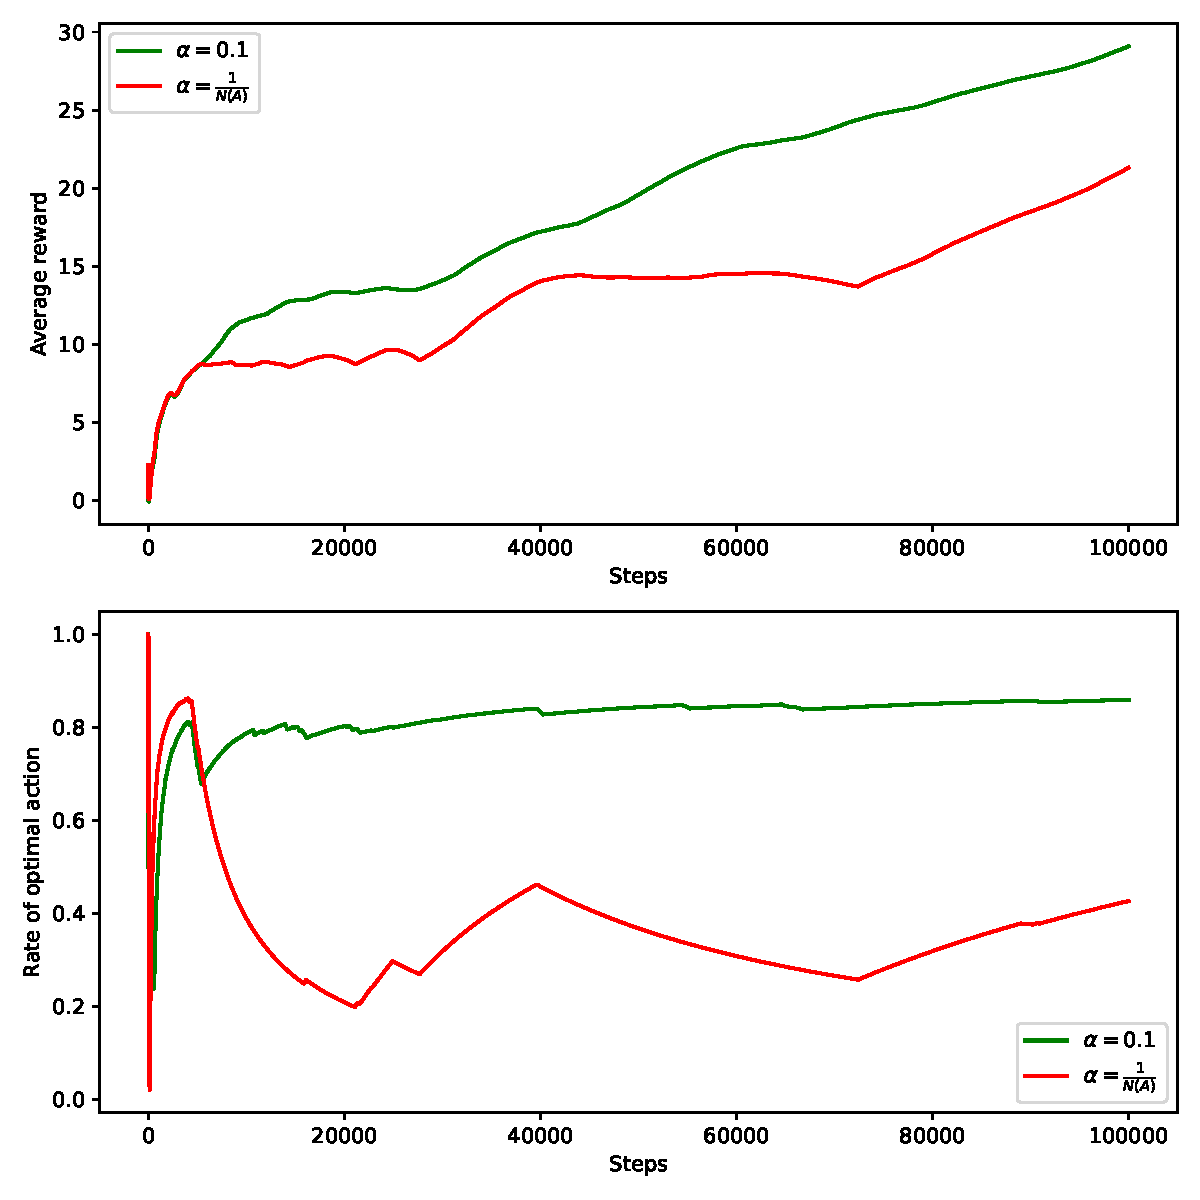
\includegraphics[width=\textwidth, angle=0]{chapters_latex/figures/ex_02_05.pdf}


\textbf{Exercise 2.6: Mysterious Spikes} \\
The results shown in Figure 2.3 should be quite reliable
because they are averages over 2000 individual, randomly chosen 10-armed bandit tasks.
Why, then, are there oscillations and spikes in the early part of the curve for the optimistic
method? In other words, what might make this method perform particularly better or
worse, on average, on particular early steps?\\

\textbf{Solution:}\\
The agent might choose the optimal action correctly, then through chance it could receive high rewards initially, so it will choose it many times, thus increasing the \% Optimal rate. After a while, again by chance, its estimate of the reward could decrease, so it would choose another suboptimal action, and the \% Optimal action would decrease. \\


\textbf{Exercise 2.7: Unbiased Constant-Step-Size Trick} \\
In most of this chapter we have used
sample averages to estimate action values because sample averages do not produce the
initial bias that constant step sizes do (see the analysis leading to (2.6)). However, sample
averages are not a completely satisfactory solution because they may perform poorly
on nonstationary problems. Is it possible to avoid the bias of constant step sizes while
retaining their advantages on nonstationary problems? One way is to use a step size of
\begin{equation}
    \beta_t \doteq \alpha / \bar{o}_t,
\end{equation}
where $\alpha > 0$ is a conventional constant step size and $\bar{o}_t$ is a trace of one that starts at 0:
\begin{equation}
    \bar{o}_{t+1} = \bar{o}_t + \alpha (1 - \bar{o}_t)
\end{equation}
for $t \geq 1$ and with $\bar{o}_1 \doteq \alpha$. \\

Carry out an analysis like that in (2.6) to show that $Q_n$ is an exponential recency-weighted average without initial bias.\\

\textbf{Solution:}\\

$\bar{o}_{t+1} = \bar{o}_t + \alpha (1 - \bar{o}_t) = \bar{o}_t(1-\alpha) + \alpha $\\

\begin{equation}
    \begin{aligned}
        \bar{o}_{1} &= \alpha \\
        \bar{o}_{2} &= \alpha + \alpha(1- \alpha) = 2\alpha - \alpha^2 \\
        \bar{o}_{t} &= \sum_{i=1}^{t} \alpha (1-\alpha)^{t-i}\\
        &=1-\left(1-\alpha\right)^{t}\\
    \end{aligned}
\end{equation}

\begin{equation}
    \begin{aligned}
        Q_{n+1} &= Q_n + \beta_n \left[ R_n - Q_n \right] \\
        &= Q_n + \frac{\alpha}{1-\left(1-\alpha\right)^{n}} \left[ R_n - Q_n \right] \\
        %&= \left( \prod_{i=1}^{n} (1-\beta_i) \right) Q_1 + \sum_{i=1}^{n} \beta_i R_i \prod_{k=i+1}^{n} (1-\beta_k) \\ 
        %&= \left( \prod_{i=1}^{n} (1-\alpha / \bar{o}_i) \right) Q_1 + \sum_{i=1}^{n} \alpha / \bar{o}_i R_i \prod_{k=i+1}^{n} (1-\alpha / \bar{o}_k) \\
    \end{aligned}
\end{equation}

The $\beta_n$ is decreasing, so it is recency-weighted. The contribution of the initial estimate $Q_1$ diminishes to zero as $t$ increases, the system effectively forgets the initial bias after a sufficient number of updates.\\

\textbf{Exercise 2.8: UCB Spikes}\\
In Figure 2.4 the UCB algorithm shows a distinct spike
in performance on the 11th step. Why is this? Note that for your answer to be fully
satisfactory it must explain both why the reward increases on the 11th step and why it
decreases on the subsequent steps. Hint: If $c = 1$, then the spike is less prominent.\\

\textbf{Solution:}

At the timesteps $t \leq 10$ there is always an action $a$ for which $N_t(a) = 0$, so the agent will always choose that action. After the 10th step the agent will choose greedily so the average reward increases. After some timesteps the uncertainty term of some other action overtakes the previously chosen action, and the agent starts to explore again, so the average reward decreases.\\

\textbf{Exercise 2.9}\\
Show that in the case of two actions, the soft-max distribution is the same
as that given by the logistic, or sigmoid, function often used in statistics and artificial
neural networks.\\

\textbf{Solution:}\\

\begin{equation}
    \begin{aligned}
        P(A_t = 1) &= \frac{e^{H_t(1)}}{\sum_{b=1}^{2} e^{H_t(b)}} = \frac{e^{H_t(1)}}{e^{H_t(1)} + e^{H_t(0)}} = \frac{1}{1 + e^{-(H_t(1)-H_t(0))}} \\
        &= \sigma(H_t(1)-H_t(0))
    \end{aligned}
\end{equation}


\textbf{Exercise 2.10}\\
Suppose you face a 2-armed bandit task whose true action values change
randomly from time step to time step. Specifically, suppose that, for any time step,
the true values of actions 1 and 2 are respectively 10 and 20 with probability 0.5 (case
A), and 90 and 80 with probability 0.5 (case B). If you are not able to tell which case
you face at any step, what is the best expected reward you can achieve and how should
you behave to achieve it? Now suppose that on each step you are told whether you are
facing case A or case B (although you still don't know the true action values). This is an
associative search task. What is the best expected reward you can achieve in this task,
and how should you behave to achieve it?\\

\textbf{Solution}\\
If we can't differentiate the 2 cases:\\
Suppose the agent chooses action 1 with probability $p$. Then the expected reward is:
\begin{equation}
    \begin{aligned}
    \mathbb{E}[R] &= P(A) \cdot \left( p R_A(1) + (1-p)  R_A(2) \right) + 
                    P(B) \cdot \left( p R_B(1) + (1-p)  R_B(2) \right)\\
        &= 0.5 (10p + 20(1-p)) + 0.5 (90p + 80(1-p)) \\
        &= 50
    \end{aligned}
\end{equation}

If we \emph{can} differentiate the 2 cases:\\
We want to maximize the reward, so in case A the agent should choose action 2 and in case B it should choose action 1.   
\begin{equation}
    \begin{aligned}
    \mathbb{E}[R] &= P(A) \cdot R_A(2) + P(B) \cdot R_B(1) \\
        &= 0.5 \cdot 20 + 0.5 \cdot 90 \\
        &= 55
    \end{aligned}
\end{equation}


\textbf{Exercise 2.11 (programming)}\\
Make a figure analogous to Figure 2.6 for the nonstationary
case outlined in Exercise 2.5. Include the constant-step-size $\varepsilon$-greedy algorithm with
$\alpha = 0.1$. Use runs of 200,000 steps and, as a performance measure for each algorithm and
parameter setting, use the average reward over the last 100,000 steps.\\

\textbf{Solution:}\\
See the notebook. \\
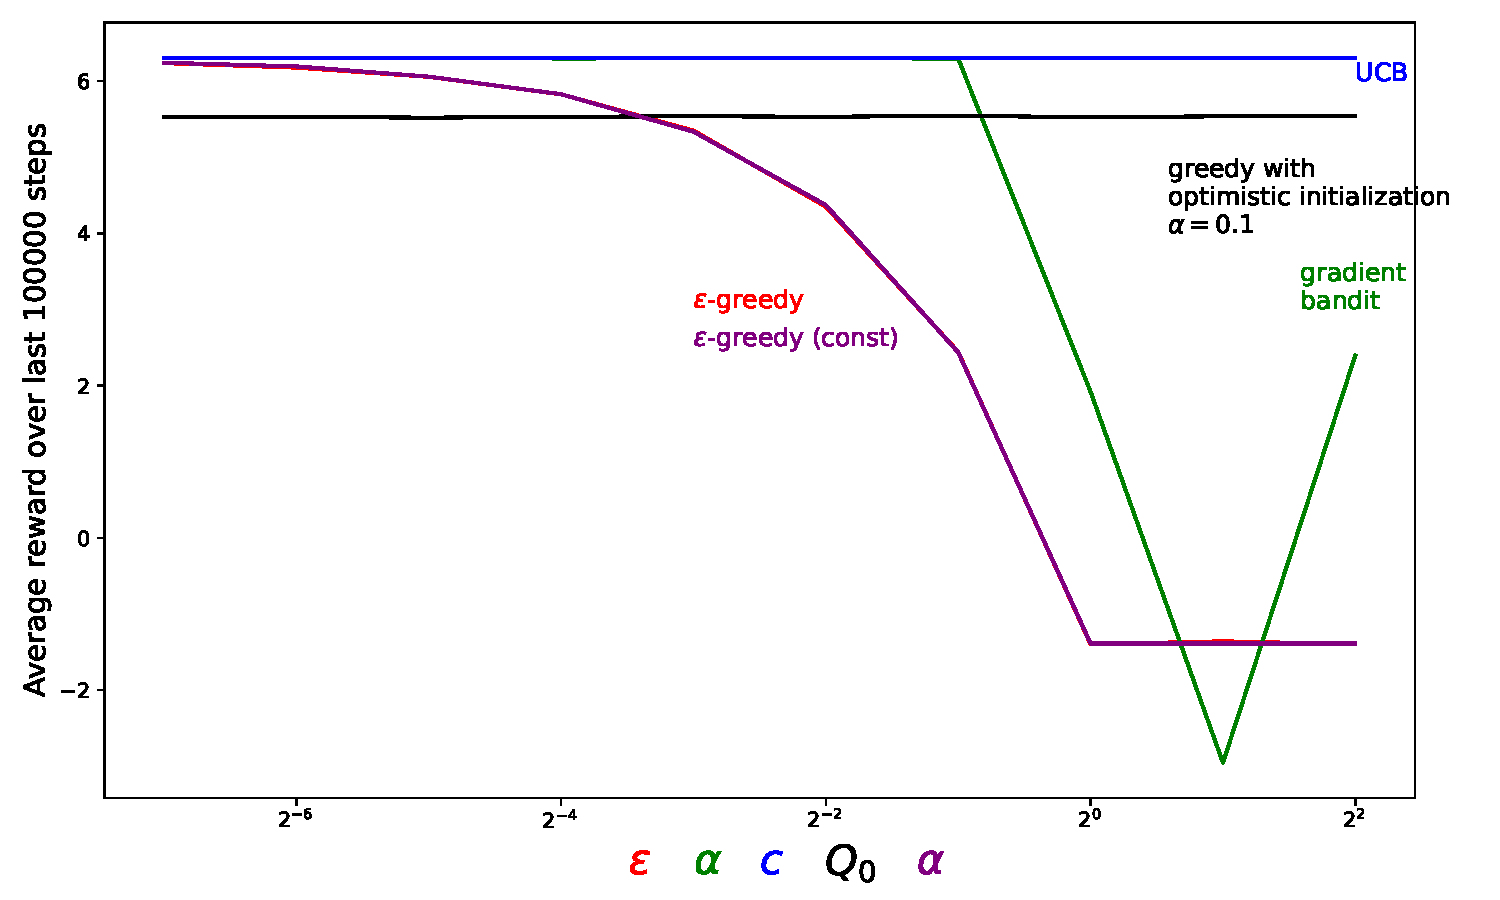
\includegraphics[width=\textwidth, angle=0]{chapters_latex/figures/ex_02_11_reward.pdf}
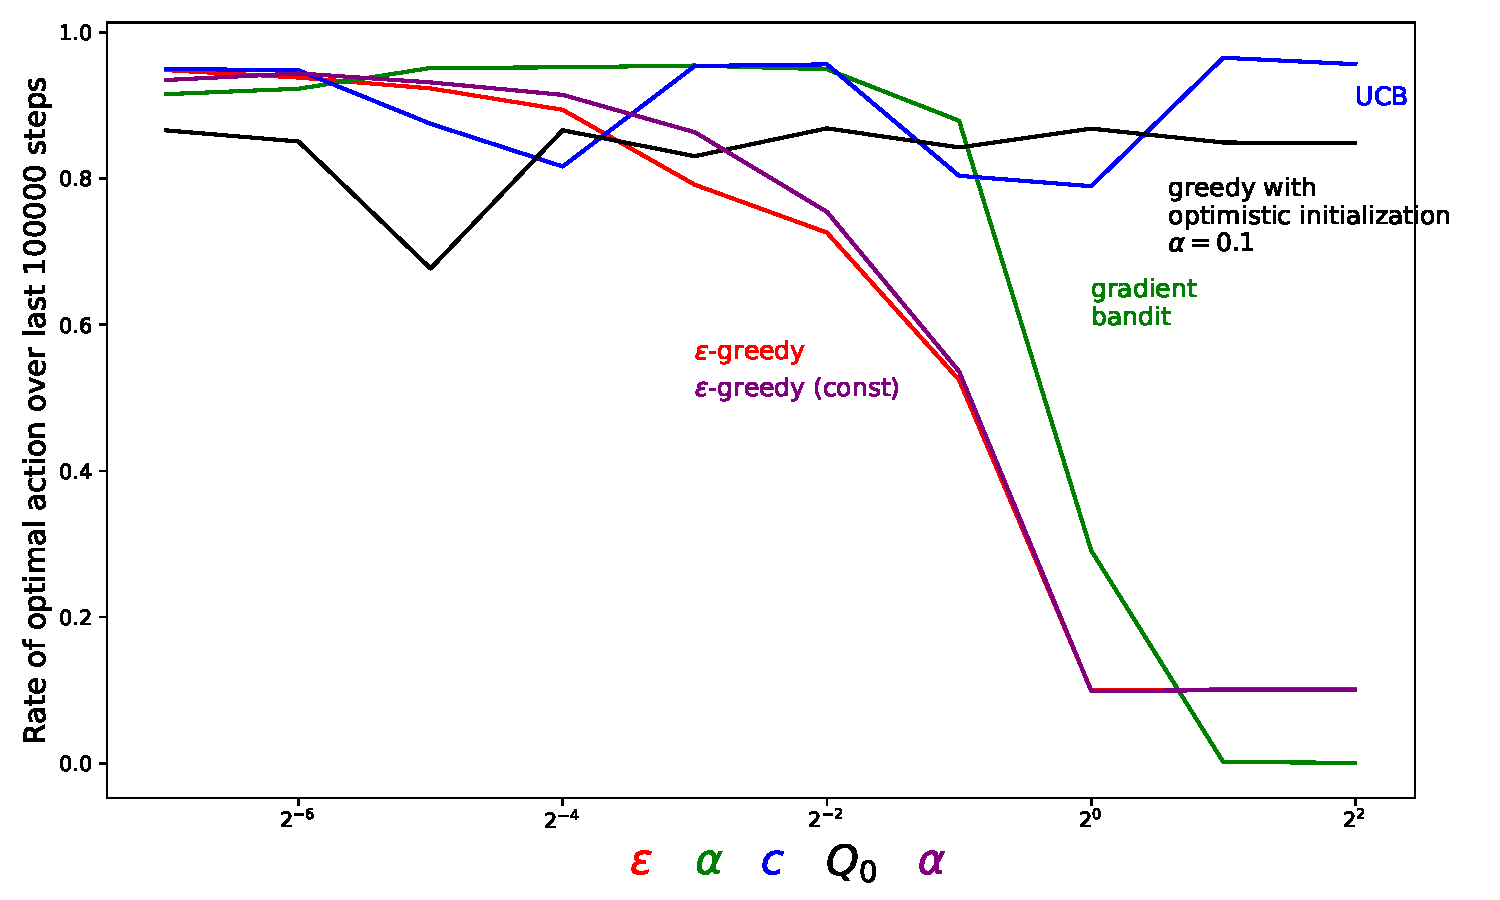
\includegraphics[width=\textwidth, angle=0]{chapters_latex/figures/ex_02_11_rate.pdf}
